\chapter{Implementation}

This chapter describes the design and implementation of a new service adding support for running workflows on cloud, with the specific target infrastructure being AWS EC2 machines. The deployment, configuration and lifecycle management of the underlying nodes executing the workflow should be transparent to the user, who is only required to provide his credentials to an AWS account.

In accordance with the considerations presented in Chapter \ref{DesignChapter} about the architecture and implementation details of both OpenMOLE and GridScale, we take a layered approach in adding support for a new cloud environment.

The first part of the chapter discusses the approach taken to bootstrap and configure a cluster consisting of EC2 machines. The cluster needs to be coordinated by a scheduler that can take job submissions and distribute them for execution.

We then proceed to analyse the integration of the cloud service with the overall OpenMOLE application. Here we treat issues such as triggering the teardown of the cluster depending on the batch submission activity and the inherent differences between the new cloud environment and the already existing types of environments.

Although we focus on deployment on AWS, the same high-level technique can easily be extended to support other cloud providers, so at the end of the chapter we briefly discuss the details of adding support for the Google Compute Engine infrastructure.

Throughout the chapter, we motivate choices made along the development process and detail problems or advantages of alternative approaches. Since the main challenge of the implementation is reliably wiring together different libraries, command line tools and cloud services, we favour the use of diagrams and code listings to show the interaction between core system components.

\section{GridScale AWS Module}

As explained in Section \ref{GridScaleSection}, access to each target environment in GridScale is implemented via a module. For the purpose of implementing an AWS module, we need to provide each of the four components: a \textit{Job Description}, a \textit{Job Service}, a \textit{Storage} interface and an \textit{Authentication} method.

\subsection{Design Motivation}

The initial idea was to simply implement an AWS specific version of each component. This is though not necessary, as we can reuse some of the already existing components from other modules and GridScale in fact encourages this approach through its modular packaging using OSGi bundles.

In particular, GridScale already supports cluster environments managed by specific schedulers. By building a cluster from a set of machines provisioned from AWS and configuring to emulate the required behaviour, we are able to partially delegate the job management work to an already functional cluster job service. This means that, in contrast with a regular cluster service that acts as a DAO\footnote{Data Access Object} for an existing infrastructure, we also need to provide interface methods through which users of the library can manage the lifecycle of the deployed cluster. We argue that this is a sane choice from an engineering perspective, since we are already familiar with reliable supported schedulers like SGE and SLURM.

The type of the job description depends on the job service, since it performs a translation to a script that can sent to the scheduler. Therefore, forwarding the submission and monitoring methods to a cluster service as discussed above implies that we need to directly use the description corresponding to the job service.

As long as we can deploy a cluster with a filesystem shared across the network, the \verb|SSHStorage| trait allows accessing the same data volume for the master and slave nodes. EC2 instances can be backed up by either EBS volumes or internal storage, but the solution of installing NFS on the cluster is agnostic to the underlying storage choice and enables using a wide range instance types.

Authentication is indeed based on the AWS credentials stored locally by the user and requires a new model. However, the standard authentication implementation relying on SSH keys can still be reused as a lower layer of this new implementation in order to access the master node that controls the job submission queue.

External applications make use of the AWS module by instantiating an \verb|AWSJobService|, which publicly exposes the following methods:

\begin{itemize}
	\item \verb|start| launches and configures a job submission cluster to be used by the service.
	\item \verb|close| completely tears down the job cluster.
	\item \verb|submit|, \verb|cancel|, \verb|state| and \verb|purge| fulfil their regular functions within the service.
\end{itemize}

Listing \ref{AWSJobService} shows an example usage of the service. The service takes as parameters the region the job should run in, as well as the number of EC2 instances that the service should create under the \verb|clusterSize| parameter. The other authentication-related parameters are discussed in \ref{CoordinatorNodeSection} and \ref{StarClusterConfigurationSection}.

\begin{listing}[h]
	\centering
	\begin{minipage}{11.8cm}
		\begin{minted}[frame=single,framesep=2mm,baselinestretch=1.11,fontsize=\small,linenos]{scala}
val awsService = AWSJobService(AWSJobService.Config(
    region = "eu-west-1",
    awsUserName = "adrian",
    awsCredentialsPath = "/Users/adrian/.aws/credentials.csv",
    awsUserId = "434676269080",
    awsKeypairName = "gridscale",
    privateKeyPath = "/Users/adrian/.ssh/id_rsa",
    clusterSize = 1))

awsService.start()

val description = new AWSJobDescription {
  def executable = "/bin/sleep"
  def arguments = "5"
  def workDirectory = aws.home
}

val job = awsService.submit(description)
while (awsService.state(job) != Done) {
  Thread.sleep(WAIT_TIME)
}

awsService.purge(job)
awsService.close()
		\end{minted}
	\end{minipage}
	\caption{Submitting a job to the cloud using the AWS module.}
	\label{AWSJobService}
\end{listing}

\vspace{-5mm}
\subsection{Cluster Deployment}

The design of the module presented above outlines the requirement for a system that can create clusters of AWS EC2 machines and configure them with a job scheduler and a shared filesystem across all nodes.

\subsubsection{Tool Choice}

During the investigations in Section \ref{ClusterDeployment}, we found that most cost-efficient tools and frameworks for creating the cluster are StarCluster, Elasticluster and Jclouds. The main reason for excluding Mesosphere DC/OS was that it is generally heavyweight and requires running more expensive machines to power the cluster. CfnCluster was dismissed for being to reliant on the AWS software stack, which incurs various extra costs for operations that can easily be performed without Amazon resources.

Jclouds allows mounting various cloud storage devices, but it did not fit our use case since it does not have built-in support for NFS installations. Although Elasticluster can perform all the required tasks, we opted for StarCluster as the cloud deployment tool, since it also provides a load balancer that can be used to optimize the cost or run time of a workflow.

\subsubsection{Coordinator Node} \label{CoordinatorNodeSection}

The choice for StarCluster raises the problem that it is only offered as a command line tool and it needs to be on the machine it is run on. Although most cluster orchestration tools require manual installation and interaction, forcing the user of the library to install an external is both unreasonable and impractical from GridScale's perspective. 

An initial idea could have been running a Docker container with StarCluster, but we can, once again, not assume the presence of a Docker engine on the user's machine.

The solution we picked was to simply create an EC2 instance with StarCluster already installed. We call this particular instance the cluster \textit{coordinator} or \textit{orchestrator}, since it controls the whole cluster activity by executing the StarCluster commands to operate it. 

The coordinator is launched using Jclouds within the \verb|start| method of the \verb|AWSJobService| created on the local machine. Its configuration is based on a prebuilt AMI with an installation of StarCluster and maintained by the developers of GridScale. After the coordinator is in a running state and its public IP address has been established, the \verb|AWSJobService| can start sending commands to it via an SSH channel. More specifically, it can emit the instruction to start a new cluster with the given name. Figure \ref{CoordinatorSetup} illustrates this whole process.

\begin{figure}[h]
	\centering
		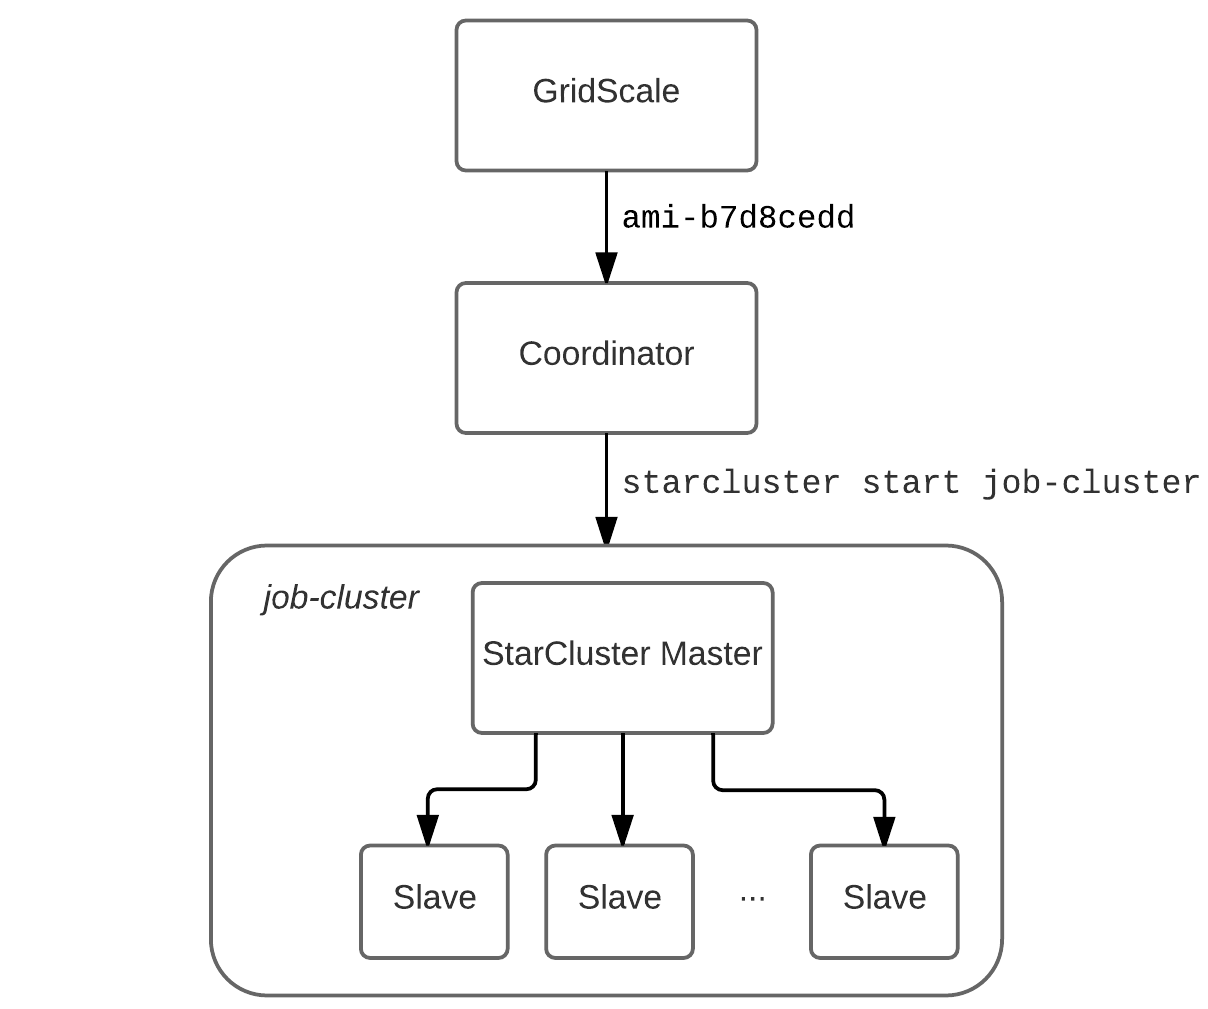
\includegraphics[width=0.87\linewidth]{CoordinatorSetup.png}
	\caption{Creating a new cluster using a proxy coordinator node and StarCluster.}
	\label{CoordinatorSetup}
\end{figure}

In order to start the coordinator node, Jclouds needs to authenticate the user. Although Amazon encourages using IAM\footnote{Identity Access Management} roles for authentication, Jclouds requires the master access key ID and secret key corresponding to the account. These are stored in the file pointed to by the \verb|awsCredentialsPath| parameter and can be downloaded by the user from the Security Credentials page in the AWS Console \cite{AWSCredentials}.

Although it might seem that introducing a proxy node for passing StarCluster commands is inefficient, the actual overhead is minimal. The reason for the limited impact is that StarCluster is only explicitly invoked during the initialisation and destruction of the cluster. All job scheduling interactions with the job submission controller bypass the coordinator, since the job service can obtain the address of the master node and send it jobs directly.

\subsubsection{StarCluster Configuration} \label{StarClusterConfigurationSection}

\subsection{SGE Delegation}

\subsection{Resource Mapper}

\subsection{GCE Version}

\section{OpenMOLE AWS Environment}

\todo[inline]{Talk about how the NFS of the job service enables sharing the runtime across execution nodes.}